\documentclass[a4paper, 12pt,oneside]{article} 
%\documentclass[a4paper, 12pt,oneside,draft]{article} 
\usepackage{preamble_bis}
%--------------------- ACTUAL FILE ---------------------- %
\begin{document} 
%%%
	\begin{titlepage}
    \newcommand{\HRule}{\rule{\linewidth}{0.5mm}} % Defines a new command for the horizontal lines, change thickness here
    
    \center  % Center everything on the page
     
    %----------------------------------------------------------------------------------------
    %   HEADING SECTIONS
    %----------------------------------------------------------------------------------------
    
    \vspace{3cm}
    \textsc{\LARGE École polytechnique fédérale de Lausanne}\\[1.5cm] % Name of your university/college
    
    \textsc{\Large Project N$^\circ$2 Report}\\[0.5cm] % Major heading such as course name
    \textsc{\large Randomized Nystr\"om
    }\\[0.5cm] % Minor heading such as course title
    
    %----------------------------------------------------------------------------------------
    %   TITLE SECTION
    %----------------------------------------------------------------------------------------
    
    \HRule \\[0.4cm] % line above and under the title
    
    
    % Title of your document
    
    \HRule \\[1.5cm]
     
    %----------------------------------------------------------------------------------------
    %   AUTHOR SECTION
    %----------------------------------------------------------------------------------------
    
    \begin{minipage}{0.4\textwidth}
    \begin{flushleft} \large
    
    \emph{Authors:}\\
    Tara \textsc{Fjellman}\\
    Amal \textsc{Seddas}\\
    
    
    
    
    \end{flushleft}
    \end{minipage}
    ~
    \begin{minipage}{0.4\textwidth}
    \begin{flushright} \large
    
    \emph{Professor:} \\
    Laura \textsc{Grigori
     }\\
    \end{flushright}
    \end{minipage}\\[10cm]
    %
    
    
    %----------------------------------------------------------------------------------------
    %   LOGO SECTION
    %----------------------------------------------------------------------------------------
    
    
\includegraphics[width=0.4\linewidth]{Logo-1 .pdf}\\[1cm] 
    % Include a department/university logo - this will require the graphicx package
     
    %----------------------------------------------------------------------------------------
    
    \vfill % Fill the rest of the page with whitespace
    
    \end{titlepage} 
	% Add titlepage
	\clearpage
	\tableofcontents
	\thispagestyle{empty}
	% Add table of contents
	\clearpage
	\pagenumbering{arabic}
	\setcounter{page}{1}

	\section{Introduction}
	In this project, we study the randomized Nyström approximation algorithm for the low-rank approximation of a positive-semidefinite matrix $A \in \mathbb{R}^{n \times n}$. There are several important applications for this theory, such as image processing, PCA, or solving integral equations. However, the most common practical setting are kernel methods for large-scale machine-learning problems. Since these algorithms scale at least quadratic in the number of data points, low-rank approximations are essential to obtain reasonable storage usage and computational costs.
	
	The randomized Nyström approximation is based on a random sketching matrix $\Omega \in \mathbb{R}^{n \times l}$ and the formula:
	\begin{equation*}
	A_{N y s t}=(A \Omega)\left(\Omega^T A \Omega\right)^{\dagger}\left(\Omega^T A\right)
	\end{equation*}
	where $l \ll n$ is the sketching dimension and $\left(\Omega^T A \Omega\right)^{\dagger}$ denotes the pseudo-inverse. In particular, the algorithm we used computes a fixed-rank $k \leq l$ approximation by truncating the sketched matrix $A_{N y s t}$. Our goal is to efficiently parallelize this alogrithm. Key aspects of our investigations are numerical stability, scalability, performance (in terms of runtime), and the approximation of the leading $k$ singular values of $A$.
	\section{Randomized Nyström low rank approximation}
	The goal of the Randomized Nystr\"om Algorithm is to represent a given matrix $A \in \mathbb{R}^{n \times n}$ by some lower rank $k<n$ approximation. The starting point of the algorithm is a rank-$\ell$ approximation of $A$, in the form
	\[
	A_{Nyst} := (A\Omega)(\Omega^T A \Omega)^{\dagger}(\Omega^T A) \in \mathbb{R}^{n \times n},
	\]
	where $(\Omega^T A \Omega)^\dagger$ is the pseudoinverse of $\Omega^T A \Omega$ and $\Omega \in \mathbb{R}^{n \times \ell}$ is a sketching matrix. We assume $k < \ell < n$. To further reduce the rank of $A_{Nyst}$ to $k$, we have two choices: approximate only the core matrix $\Omega^T A \Omega$ or the whole $A_{Nyst}$. In this project, we focus on the second approach. Algorithm \ref{alg:nystrom} shows how this can be achieved.

\begin{algorithm}
\caption{Randomized Nystr\"om approximation using the Cholesky decomposition}
\label{alg:nystrom}
\begin{algorithmic}[1]
  \State Let $C = A\Omega$ and $B = \Omega^T C$.
  \State Compute the Cholesky decomposition: $B = LL^T$.
  \State Solve the linear system using back substitution: $Z = C(L^T)^{-1}$.
  \State Perform QR decomposition: $Z = QR$.
  \State Compute the singular value decomposition (SVD) of $R$ and truncate:
  \[ R = U \Sigma V^T \approx \tilde{U}_k \tilde{\Sigma}_k \tilde{V}_k^T. \]
  \State Set $\tilde{U}_k = Q\tilde{U}_k$ (or equivalently $\tilde{U}_k = Z\tilde{V}_k\tilde{\Sigma}_k^{-1}$) and return $\tilde{U}_k \tilde{\Sigma}_k^2 \tilde{U}_k^T \approx A_{Nyst}$.
\end{algorithmic}
\end{algorithm}

To show why the result of Algorithm \ref{alg:nystrom} is in fact a rank-$k$ approximation of $A_{Nyst}$, we write
\begin{align*}
\tilde{U}_k \tilde{\Sigma}_k^2 \tilde{U}_k^T &= Q\tilde{U}_k \tilde{\Sigma}_k \tilde{\Sigma}_k^T \tilde{U}_k^T Q^T \\
&\approx QRR^T Q^T = ZZ^T = A\Omega(L^T)^{-1}(L^T)^{-1}\Omega^T A^T \\
&= A\Omega(LL^T)^{-1}\Omega^T A^T = A(\Omega^T A \Omega)^{\dagger}\Omega^T A^T.
\end{align*}

However, here we have the inverse of $\Omega^T A \Omega$ instead of its pseudoinverse. Unfortunately, Algorithm \ref{alg:nystrom} fails in Step 2 if $\Omega^T A \Omega$ is numerically singular. In this case, as in \cite{reference}, we replace $L$ by a square root of $B$ in SVD form. Specifically, we write $B = U_B \Sigma_B U_B^T$ (since $B$ is SPSD), and set $L = U_B \sqrt{\Sigma_B} U_B^T$. By construction, we have
\[
LL^T = U_B \sqrt{\Sigma_B} U_B^T (U_B \sqrt{\Sigma_B} U_B^T)^T = U_B \Sigma_B U_B^T = B.
\]
We then replace $(L^T)^{-1}$ with $(L^T)^\dagger$. This can be simply calculated as
\[
(L^T)^\dagger = (U_B \sqrt{\Sigma_B} U_B^T)^\dagger,
\]
where $\sqrt{\Sigma_B}$ is a diagonal matrix whose entries are given by
\[
(\sqrt{\Sigma_B})_{i,i} = \begin{cases} \frac{1}{(\sqrt{\Sigma_B})_{i,i}} & \text{if } (\sqrt{\Sigma_B})_{i,i} \neq 0, \\
0 & \text{otherwise.} \end{cases}
\]
\section{Sketching and Sketching Matrices}

In this section, we provide a detailed overview of sketching and the sketching matrices utilized in this project. The concept of sketching involves transforming a high-dimensional matrix $A \in \mathbb{R}^{n \times n}$ into a lower-dimensional representation $A\Omega$, where $\Omega \in \mathbb{R}^{n \times \ell}$ is a tall and skinny sketching matrix. The goal of sketching is to embed the high-dimensional data into a reduced-dimensional space while preserving the essential geometric properties of the data.

More formally, given any two vectors $x$ and $y$ in the high-dimensional space, their sketched counterparts $\hat{x}$ and $\hat{y}$ should approximately preserve their inner product:
\begin{equation}\label{eq:1}
\left| \langle \hat{x}, \hat{y} \rangle - \langle x, y \rangle \right| \leq \varepsilon \|x\|_2 \|y\|_2 \tag{2}
\end{equation}
where $\varepsilon > 0$ is a small approximation error. However, achieving this exact preservation for all $x$ and $y$ is generally infeasible due to the reduced dimensionality $\ell$. Instead, $\Omega$ is typically regarded as a random matrix, ensuring that \cref{eq:1} holds with high probability $1 - \delta$, where $\delta < 1$.

In this project, we employ two specific types of sketching matrices:
\subsection{Gaussian sketching }
The Gaussian sketching matrix is random projection method in which the entries of the sketching matrix $\Omega$ are drawn independently from a standard normal distribution. Mathematically, it is defined as:
\[
\Omega_{ij} \sim \mathcal{N}(0, 1).
\]
%where $\Omega \in \mathbb{R}^{n \times \ell}$, and $\ell$ represents the reduced dimensionality of the sketch.
% this is not necessary, as we already defined Omega above

This method is such that for an input matrix $A \in \mathbb{R}^{n \times d}$ and for any vector $x \in \mathbb{R}^l$:
\[
(1 - \varepsilon)\|A x\|_2^2 \leq \|A \Omega x\|_2^2 \leq (1 + \varepsilon)\|A x\|_2^2,
\]
with high probability, where $\varepsilon > 0$ is a small approximation error. This property ensures that pairwise distances between points in the projected space are approximately preserved.

The Gaussian sketching matrix can also be viewed as a random transformation that approximately satisfies the following subspace embedding property for any subspace $T \subseteq \mathbb{R}^l$:
\[
(1 - \varepsilon) \|v\|_2^2 \leq \|\Omega v\|_2^2 \leq (1 + \varepsilon) \|v\|_2^2, \quad \forall v \in T.
\]

\subsection{Subsampled Randomized Hadamard Transform (SRHT)}
BSRHT is a version of the Subsampled Randomized Hadamard Transform (SRHT) specifically designed for distributed architectures. For $n$ being a power of two, the SRHT can be defined as
\[
\Omega^T = \sqrt{\frac{n}{\ell}} RHD,
\]
where: $H \in \mathbb{R}^{n \times n}$ is the normalized Walsh-Hadamard matrix; $D \in \mathbb{R}^{n \times n}$ is a diagonal matrix with i.i.d. random variables $\sim \text{Uniform}(\pm 1)$; and $R \in \mathbb{R}^{\ell \times n}$ is a subset of $\ell$ randomly sampled rows from the $n \times n$ identity matrix.

Now, for $P$ different processors, BSRHT can be constructed block-wise from the SRHT as:
\[
\Omega^T = \begin{pmatrix} \Omega_1^T \\
\Omega_2^T \\
\vdots \\
\Omega_P^T \end{pmatrix} = \sqrt{\frac{n}{P\ell}} \begin{pmatrix} D_{L1} & \cdots & D_{LP} \end{pmatrix}
\begin{pmatrix}
RH & \cdots & 0 \\
\vdots & \ddots & \vdots \\
0 & \cdots & RH
\end{pmatrix}
\begin{pmatrix} D_{R1} & \cdots & 0 \\
\vdots & \ddots & \vdots \\
0 & \cdots & D_{RP} \end{pmatrix}, \tag{2}
\]
with: $H \in \mathbb{R}^{n/P \times \ell/P}$ being the normalized Walsh-Hadamard matrix; $D_{Li} \in \mathbb{R}^{n/P \times n/P}$, $D_{Ri} \in \mathbb{R}^{n/P \times n/P}$ being diagonal matrices with i.i.d. Rademacher entries $\pm 1$; and $R \in \mathbb{R}^{\ell \times n/P}$ being a uniform sampling matrix, sampling along the rows.

This structure is particularly suited for distributed computations, as it allows for parallelism while maintaining the theoretical properties of the SRHT.

	\section{Parallelisation}
	We parallelise the algorithm by distributing among the processors the computation of $A \Omega,\Omega^T A \Omega$, and all other matrix operations with complexities at least proportional to $n$. 
	
	The parallelisation of QR factorisation was the topic of the first project. We therefore included the relevant functions for it in the code folder. 
	
	The parallelisation of matrix products was however implemented from scratch. It was done as described in algorithm \ref{alg:parallel-matrix-product}, by distributing matrices smartly among the processors. 
	\begin{algorithm}[H]
		\caption{Computes the matrix product of two matrices $D$ and $E$ in parallel.}\label{alg:parallel-matrix-product}
		\begin{algorithmic}
		\Require $q$ is an integer and the square root of the number of processors, $D$ is an $m\times m$ matrix distributed such that processor $i$ has $D_{i//q,i\text{ mod }q}$ and $E$ is a $m\times n$ matrix distributed such that processor $i$ has $E_{i//q}$. FullProd is true if we also want to compute $E^TDE$.
		\Ensure $F=DE$ (and $G=E^TF$ too if FullProd is true). 
		\State $F_{ij} \gets P_{ij}E_j$
		\If{\text{FullProd}}
			\State $G_{ij} \gets E_i^FP_{ij}$
		\EndIf		
		\State Row-wise Sum-reduce : $F_i\gets \sum_j^q F_{ij}$
		\State Column-wise Gather on rank 0 : $F\gets [F_1^T,...,F_q^T]^T$
		\If{\text{FullProd}}
			\State Sum-reduce : $G\gets \sum_{i,j}^{q,q} G_{ij}$
		\EndIf
		\end{algorithmic}
	\end{algorithm}
	This version of the matrix product allows for a fluid computation of both the $A \Omega,\Omega^T A \Omega$ products involved in the sketching and general matrix products between two matrices $D$ and $E$ which appear in the computation of the rank-$k$ approximation. 
	
	The pseudo-code for the parallelisation of the randomized Nystr\"om algorithm is then described in algorithm \ref{alg:parallel-rand-nystrom}.
	\begin{algorithm}[htb]
		\caption{Randomized Nystr\"om algorithm. The syntax was adapted from this Overleaf example.}\label{alg:parallel-rand-nystrom}
		\begin{algorithmic}
		\Require $A$ is an $n\times n$ symmetric positive semidefinite matrix, $\Omega$ is a sketching matrix of size $n\times l$, and $k$ is the rank of the approximation
		\Ensure $[A_{N y s t}]_k$, the rank-$k$ randomized Nystr\"om approximation of $A$. 
		\State $C \gets A \Omega$
		\State $B \gets \Omega^T C$
		\State $L, \text{Failed} \gets \text{Cholesky}(B)$ \Comment{Locally on rank 0}
		\If{Failed}
			\State $U, \Lambda \gets \text{EigDecomp}(B)$ \Comment{Locally on rank 0}
			\State $B_k^{+} \gets U(:,1:k) \Lambda(1: k, 1: k)^{+} U(:, 1: k)^T$
			\State $Q, R \gets \text{QR}(C)$ \Comment{Using TSQR}
			\State $\hat{U}_k \gets Q U(:, 1:k)$ \Comment{In parallel}
			\State $[A_{N y s t}]_k \gets \hat{U}_k \Lambda(1: k, 1: k)^{+} \hat{U}_k^T$ \Comment{In parallel}
		\Else{}
			\State $Z \gets C L^{-T}$ \Comment{Computed by substitution : $(LZ^T)^T=C^T$}
			\State $Q, R \gets \text{QR}(Z)$ \Comment{Using TSQR}
			\State $U_k, \Sigma_k, V_k \gets \text{TruncSVD}(R)$
			\State $\hat{U}_k \gets Q U(:, 1:k)$ \Comment{In parallel}
			\State $[A_{N y s t}]_k \gets \hat{U}_k \Sigma^2(1: k, 1: k) \hat{U}_k^T$ \Comment{In parallel}
		\EndIf
		\end{algorithmic}
	\end{algorithm}
	%$$
	%S=\left(\begin{array}{lll}
	%S_{0} & S_{01} & S_{02} \\
	%S_{10} & S_{11} & S_{12} \\
	%S_{20} & S_{21} & S_{22}
	%\end{array}\right), \quad \Omega=\left(\begin{array}{l}
	%T_0 \\
	%T_1 \\
	%T_2
	%\end{array}\right),
	%$$
	%$$
	%B=\Omega^T A \Omega=\left(\begin{array}{lll}
	%	\Omega_1^T & \Omega_2^T & \Omega_3^T
	%	\end{array}\right)\left(\begin{array}{lll}
	%	A_{11} & A_{12} & A_{13} \\
	%	A_{21} & A_{22} & A_{23} \\
	%	A_{31} & A_{32} & A_{33}
	%	\end{array}\right)\left(\begin{array}{l}
	%	\Omega_1 \\
	%	\Omega_2 \\
	%	\Omega_3
	%	\end{array}\right)
	%$$
	%with processor $i$ having the $i$-th row of $S$ and the $i$-th block row of $T$. Then
	%$A \Omega,\Omega^T A \Omega$ multiplications were implemented 
	%The matrix $A$ is distributed among processors by using a two-dimensional block distribution while the matrix $\Omega$ is distributed using a block row distribution. The parallelization of the algorithm is implemented in the following way:
	%Describe how you parallelize randomized Nyström and provide pseudo-code of the parallel algorithm. For the parallelization, the matrix $A$ should be distributed among processors by using a two-dimensional block distribution while the matrix $\Omega$ should be distributed using a block row distribution. You can consider that the number of processors is a power of 2 such that you can easily distribute the matrices among processors. For example, when $P=\sqrt{P} \times \sqrt{P}=9$, the matrices $A$ and $\Omega$ are distributed as:
	\section{Experimental procedure}
		The presented results were obtained by running our scripts on the Helvetios cluster, by averaging over different runs to make results more robust and interpretable.
		
		In general, due to the BSRHT making use of the Hadamard transformation, $n$ was made vary as powers of $2$ only. In reality one can always zero-pad the data to ensure that the Hadamard transformation can be applied. This was however avoided for performance analysis since it would have introduced unnecessary variation in the measurements.  
		\subsection{Datasets}
		In this project, we consider two types of datasets to evaluate the performance of our methods: synthetic datasets and those derived from the MNIST dataset. For the synthetic datasets, we construct diagonal matrices with positive eigenvalues and different rates of decay for the singular values. We explore both \textit{polynomial decay} and \textit{exponential decay}, with rates categorized as \textit{slow}, \textit{medium}, and \textit{fast}. The diagonal structure allows us to easily select the singular values and define an effective rank \( R \) for the matrices. This design provides controlled conditions for studying spectral properties and their influence on algorithmic performance.

For the datasets derived from MNIST, we normalize the data to have values in the range \([0, 1]\) and use a subset of \( n \) data points. A similarity matrix is then constructed using the radial basis function (RBF), defined as:

\[
A_{ij} = e^{-\|x_i - x_j\|^2 / c^2}
\]

where \( x_i \) and \( x_j \) are data samples, and \( c \) is a tunable parameter controlling the penalty for dissimilarity. This results in a symmetric, dense \( n \times n \) matrix, where \( c \) determines how rapidly similarity decreases with distance. To ensure consistent computations, we normalize the MNIST dataset by dividing each pixel value by the maximum intensity across the dataset.

We visualize the singular value decay of these datasets in \cref{fig:singular_values}, which highlights the differences between the decay patterns for the synthetic matrices and the RBF-based similarity matrices derived from MNIST.
\begin{figure}[H]
    \centering
    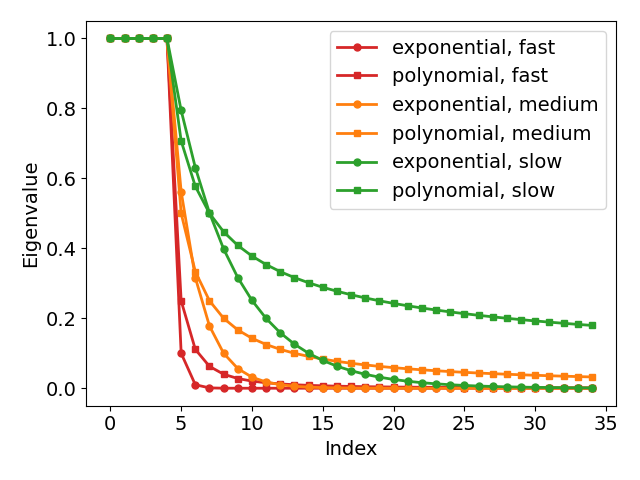
\includegraphics[width=0.45\textwidth]{synthetic_spectra.png}
    \hspace{0.02\textwidth} % Add horizontal space
    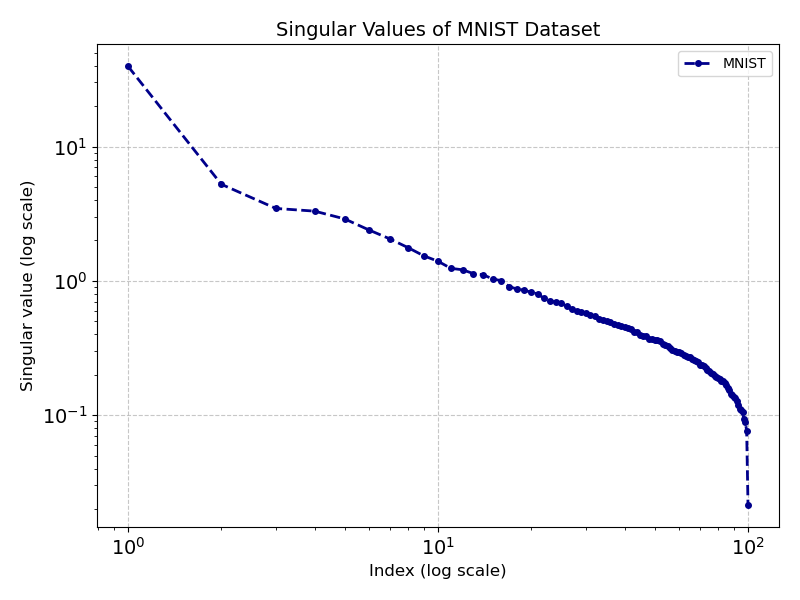
\includegraphics[width=0.45\textwidth]{mnist_singular_values_darkblue.png}
    \caption{Singular value decay of synthetic matrices (left) and the MNIST-based similarity matrix (right).}
    \label{fig:singular_value_comparison}
\end{figure}
		\subsection{Stability analysis}
		
		In this section, we investigate how our algorithm performs from a numerical point of view. The metric we use to assess the quality of our results is the trace relative error, defined as
\[
\frac{\|A - A_{\text{Nyst}}\|_*}{\|A\|_*},
\]
where \(\|\cdot\|_*\) is the nuclear norm. Since the nuclear norm is the sum of the singular values, \(\|A\|_* = \sigma_1(A) + \cdots + \sigma_n(A)\), this value describes the ratio of the sum of the singular values corresponding to the approximation error of \(A_{\text{Nyst}, k}\) compared to the original matrix \(A\).

If this value is low, we have a good low-rank approximation of \(A\).

The ExpDecay dataset highlights the differences in numerical stability between Gaussian Sketch and Block SRHT. As shown in Figure~\ref{fig:expdecay}, Gaussian Sketch demonstrates a sharp and consistent decrease in relative error as the approximation rank \(k\) increases. This indicates that Gaussian Sketch is particularly effective for datasets with rapidly decaying spectra. In contrast, Block SRHT shows a more gradual reduction in relative error, suggesting that its structured embedding approach may be less adaptive in scenarios dominated by exponential decay.

\begin{figure}[H]
\centering
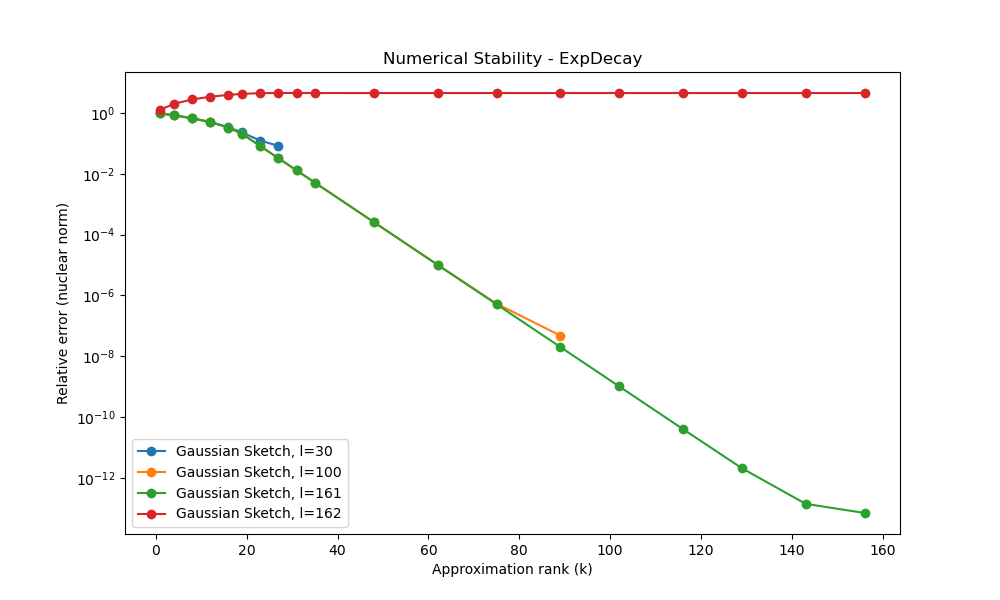
\includegraphics[width=0.8\textwidth]{ExpDecay_stability.png}
\caption{Numerical Stability Results for ExpDecay Dataset.}
\label{fig:expdecay}
\end{figure}

For the MNIST dataset, illustrated in Figure~\ref{fig:mnist}, both sketching methods display steady improvements in relative error as \(k\) increases. Gaussian Sketch achieves slightly lower errors for smaller \(k\), making it advantageous in settings with limited computational resources. However, as \(k\) grows, the performance of the two methods converges, highlighting the robustness of the Block SRHT approach. Block SRHT maintains smoother error reduction trends across all \(k\) values, reflecting its superior numerical stability and consistency on this dataset.

\begin{figure}[H]
\centering
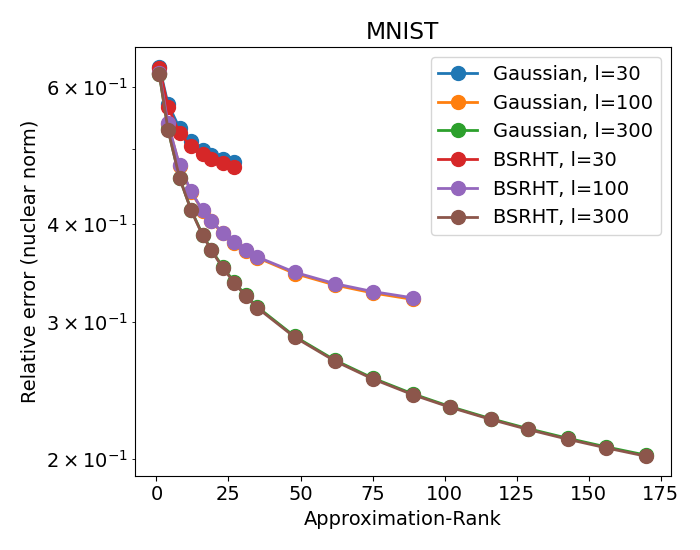
\includegraphics[width=0.8\textwidth]{MNIST_stability.png}
\caption{Numerical Stability Results for MNIST Dataset.}
\label{fig:mnist}
\end{figure}

The PolyDecay dataset, depicted in Figure~\ref{fig:polydecay}, emphasizes the strong performance of Gaussian Sketch for datasets with polynomial spectral decay. Gaussian Sketch shows a pronounced and rapid reduction in relative error as \(k\) increases, significantly surpassing Block SRHT at higher ranks. This result highlights the flexibility of Gaussian Sketch for datasets with slower-decaying eigenvalues. Meanwhile, Block SRHT demonstrates a steadier reduction in error, showcasing its robustness and reliability for consistent approximations.

\begin{figure}[H]
\centering
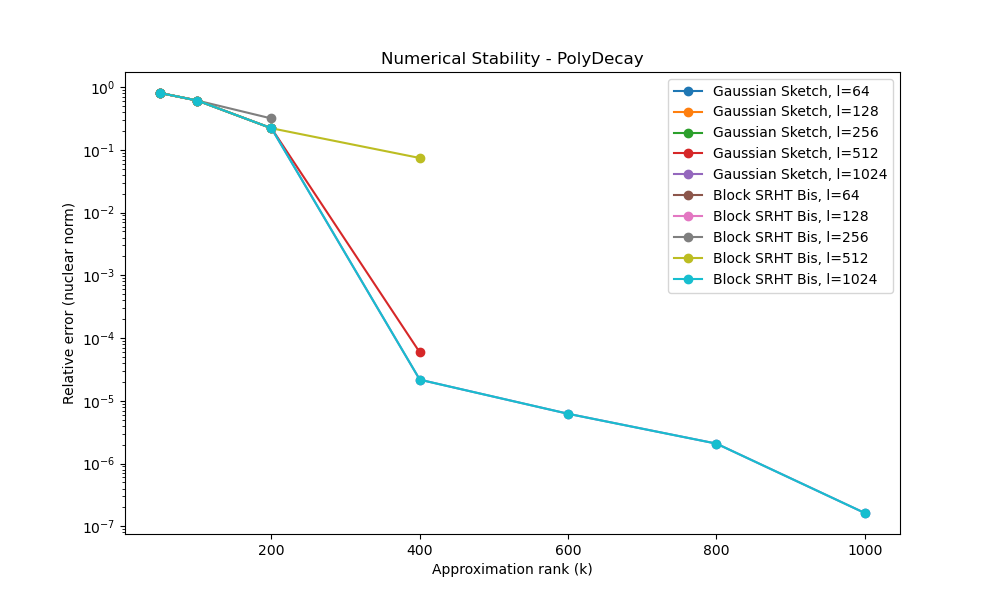
\includegraphics[width=0.8\textwidth]{PolyDecay_stability.png}
\caption{Numerical Stability Results for PolyDecay Dataset.}
\label{fig:polydecay}
\end{figure}

Overall, these results suggest that Gaussian Sketch excels in numerical accuracy, particularly for datasets with rapidly or polynomially decaying spectra. However, Block SRHT offers smoother error reduction trends and exceptional robustness, making it a reliable choice for distributed and large-scale computations. Further analysis of their computational efficiency will follow in subsequent sections.
	\subsection{Performance analysis}
		For these results to have some general relevance, we tried considering realistic values of $k$ and $l$. More specifically, $k$ was taken often around $n/20$, while $l$ was taken logaritmically spaced.
	
		When running in parallel, the number of processors was limited to values $P=2^{2s}$ with $s\in\mathbb{N}$. This was due to perfect square constraint of the parallelised matrix multiplication and the BSHRT's use of the Hadamard transform. The values of $P$ we choose were 1,4,16,64. 		
		This also meant having to take $l\le n/64$ integer for the TSQR algorithm to at least have one block-row per processor at the start of its run. We also recall that to see speed-up with parallelisation we need the matrix to be tall-skinny. To have a good speed-up for a bigger $l$, while keeping numerical stability for ill-conditioned matrices another algo should be used.
	
	
		\section{Algorithm Performance}
        \subsection{Sequential Performance}
		To explore the sequential runtimes of the implemented algorithms, we decided to do two longitudinal studies : first varying $l$ for a selected value of $n$, and then varying $n$ for a selected $l$. The associated results are represented in \ref{fig:runtimes-l-n-variation}. 

		The main feature common to both plots is that the $k$ rank approximation part of the computation represents in most cases as small minority of runtime (as expected, since it should be of order $l^3 +nk^2$). This would of course change if one were to take big values of $k$ (i.e. if the data was really information-dense).  	
		It's runtimes also do not really seem to depend on the sketching method. This makes sense given the computations are the same regardless of which sketching method was used to obtain the B and C matrices. One could probably change this if one were to fully take advantage of the structure of the matrices involved in the BSRHT method (as one could use integer-float operations instead of float-float ones). 

		Looking more closely at both figures, it is clear that different behaviours are observed as a function of $l$ and $n$. We discuss each in the following paragraphs.
		\begin{figure}[htb]       
			\centering             
				\vspace{0em}
				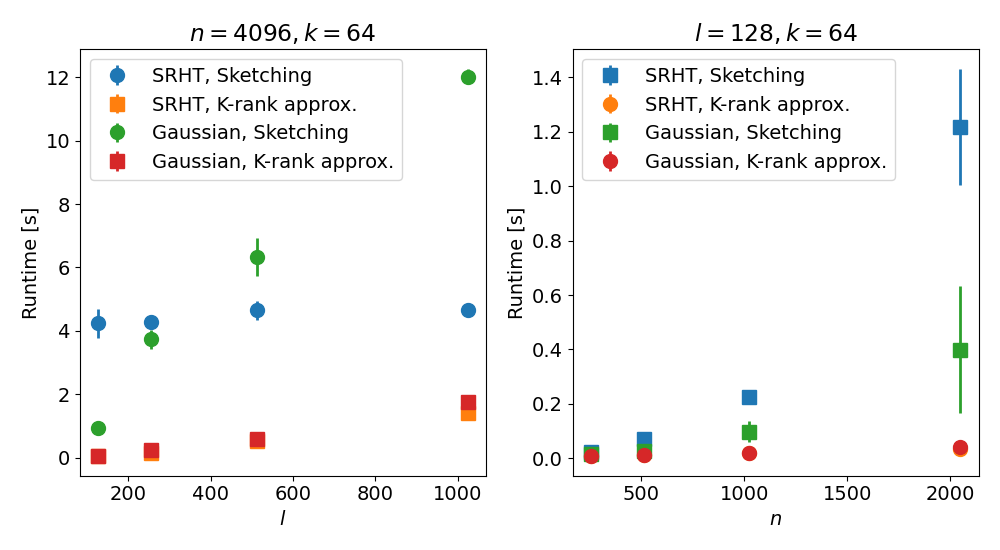
\includegraphics[width=.975\textwidth]{runtimes_l_n_variation}
				\caption{Runtimes associated to the tested sketching methods : as a function of $l$ (left) and as a function of $n$ (right). Runtimes are broken down in that associated to the computation of $A\Omega,\Omega^T A\Omega$ and that associated to the computation of the $k$ rank approximation.}
				\label{fig:runtimes-l-n-variation}
		\end{figure}
		\paragraph{$l$ variation}
		As a function of $l$ we observe extremely different behaviours from Gaussian and BSRHT sketchings. Indeed : the curve for BSRHT looks basically flat, while the Gaussian one increases steadily. This is expected given the complexities of the algorithms respectively are of order $n^2\log_2{n}$ and $nl^2 + ln^2$. This gives a great advantage in using BSRHT if we are embedding information-dense spaces as it scales much better.		

		Coming back to the $k$-rank approximation runtimes, we notice that the expected considerable increase as a function of $l$ is observed, even if as mentioned it stays relatively small when compared to the sketching runtime.
		\paragraph{$n$ variation}
		As a function of $n$ both algorithms show significant increase. BSRHT shows faster runtime growth. For $n=1024$ it seems to take twice the time, while for $n=2048$ it seems to take three times as much. This is a perfect match due to extra $\log_2(n)$ term in its complexity. This gives a considerable advantage in using Gaussian sketching when handling information-sparse within high dimensional spaces.

		As for the $k$-rank approximation runtimes, the linear increase as a function of $n$ is hard to see on the plot due to the different scale. 
        \subsection{Parallel Performance}
			We now turn to the analysis of the parallel performance. The relevant plot for this section is \ref{fig:runtimes-cores-variation}. For the sake of structure, we analyse separately the small and the large runs.
			\begin{figure}[htb]       
				\centering             
					\vspace{0em}
					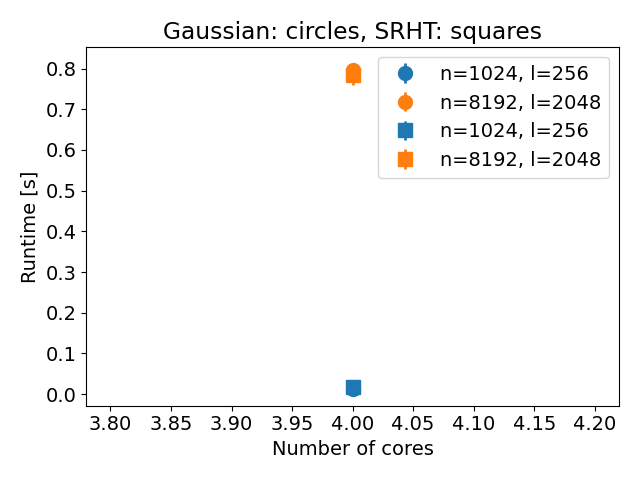
\includegraphics[width=.975\textwidth]{runtimes_cores_variation}
					\caption{Runtimes associated to the tested sketching methods as a function of the number of cores : for a ``small'' example (left) and a ``large'' one (right). Runtimes are broken down in that associated to the computation of $A\Omega,\Omega^T A\Omega$ and that associated to the computation of the $k$ rank approximation.}
					\label{fig:runtimes-cores-variation}
			\end{figure}
			\paragraph{Small run}
			For the small run we first observe that some speed-up is displayed as a function of number of cores for both sketching methods. The speed-up is quasi-linear for BRSHT, while it saturates and back-fires for Gaussian sketching, due to the communication overhead. Given that the $k$-rank approximation part of the computation is smaller, it is most affected by the cost of communication, which actually dominates all throughout the core-number sweep.   
			These behaviours are expected given that : (a) the computation is rather small to be run in parallel; (b) BRSHT is slower than Gaussian sketching for small values of $l$. 
			
			For the specific parameter values selected, Gaussian sketching is a factor $\approx 10$ faster than BRSHT (except $P=64$).
			\paragraph{Large run}
			For the large run the results are quite different. Communication is not an issue for the sketching part, meaning that quasi-linear speed-ups are observed for both methods. This means the parallelization is successful and scales well for big computations. We also observe initial speed-up for the $k$-rank approximation, though it is short-lived due to the computation still being quite small and due to that the matrix is not that tall-skinny (reducing the benefit in the QR decomposition). 
	\section{Conclusion}
	\section*{Aknowledgements}
	\section*{References}
	%\appendix
	%	\section{Runtime Estimation}\label{appendix:runtime_estimation}
%%%
\end{document} 